\documentclass[sigconf,nonacm]{acmart}

\usepackage{array}
\usepackage{iftex}
% Preview build only: if the Libertine TeX fonts are missing and XeLaTeX is used, fall back to the
% installed OpenType Libertine so the PDF looks like the ACM style. With a full TeX Live or Overleaf
% (pdfLaTeX) this block does nothing and acmart's own fonts are used.
\IfFileExists{libertine.sty}{}{%
  \ifXeTeX
    \usepackage{fontspec}
    \IfFontExistsTF{Linux Libertine O}{\setmainfont{Linux Libertine O}\setsansfont{Linux Biolinum O}}{}
    \IfFontExistsTF{Inconsolata}{\setmonofont[Scale=MatchLowercase]{Inconsolata}}{}
  \fi}
\usepackage{booktabs}
\usepackage{tikz}
\usetikzlibrary{positioning,arrows.meta,shapes.geometric,fit,calc}

\settopmatter{printfolios=true}
\renewcommand\footnotetextcopyrightpermission[1]{}
\pagestyle{plain}

\setlength{\emergencystretch}{3em}
\usepackage{xr-hyper}
\externaldocument[S-]{supplement}
\begin{document}

\title{DSL Coverage, Search Guidance and Hypothesis Construction in Symbolic Program Synthesis for ARC-AGI-2}

\author{Joy Bose}
\affiliation{%
  \institution{Hexaware Technologies}
  \city{Bengaluru}
  \country{India}}
\email{joy.bose@acm.org}

\begin{abstract}
We ask where a small, fully symbolic program-synthesis system for ARC-AGI-2 fails: in representation (does a fitting program exist?), search (can it be reached affordably?) or selection (is the right program chosen among those that fit?). The system searches short programs in a domain-specific language (DSL), keeps only programs that reproduce every training example, and prefers the shortest. On the 120 public evaluation tasks, thirteen settings over DSLs of 44, 135 and 201 primitives solve none, and for none of the tasks does any depth-2 program fit the training pairs; exhaustive merged-state search through depth 3 finds no fit on 18 randomly selected tasks, and an object-relational solver extended in three steps also solves none. Diagnostics on separate training tasks, reported in the supplement as diagnostics and not as performance, point the same way: growing the DSL gives diminishing returns, a learned primitive proposer beats random pruning but not unpruned depth-2 search, and shortest-first selection adds little. Library expansion is not representation expansion. The one qualitative change comes from a different kind of step: a task-conditioned learner that builds the structure of the rule from each task's examples, as a decision tree over per-cell features, gives the study's only public-evaluation solve, 1 of 120, and no later variant changed that count. The frozen combined solver scores 1.67 on the 240 hidden Kaggle test tasks (4 of 240 if every task counts equally). Its fits are spurious more often than flat programs, but a leave-one-pair-out check separates them well on development tasks (20 of 21 fits that pass are correct, against 15 of 79 that do not), and for none of 90 wrong development fits was another candidate tree correct, so its failures are failures of construction, not of ranking. The flat-library experiments are the clean, pre-specified evidence; the cell-tree results are exploratory and rest on a single evaluation task. Within the tested regime, the results suggest that further gains require changing how hypotheses are constructed, rather than only improving ranking or pruning within the existing DSL. We report all results, negative ones included, as a reproducible baseline.
\end{abstract}

\begin{CCSXML}
<ccs2012>
<concept>
<concept_id>10010147.10010178.10010187</concept_id>
<concept_desc>Computing methodologies~Knowledge representation and reasoning</concept_desc>
<concept_significance>500</concept_significance>
</concept>
<concept>
<concept_id>10011007.10011074.10011092.10011782</concept_id>
<concept_desc>Software and its engineering~Automatic programming</concept_desc>
<concept_significance>300</concept_significance>
</concept>
</ccs2012>
\end{CCSXML}

\ccsdesc[500]{Computing methodologies~Knowledge representation and reasoning}
\ccsdesc[300]{Software and its engineering~Automatic programming}

\keywords{ARC-AGI-2, abstraction and reasoning, program synthesis, domain-specific language, neurally guided search, description length}

\maketitle

%% ==================================================================
\section{Introduction}

The Abstraction and Reasoning Corpus (ARC) was proposed as a test of how well a system can pick up a new skill from very little data, rather than how much it has memorized~\cite{chollet2019measure}. Each task shows a few pairs of coloured grids. In every pair the output is made from the input by the same hidden rule. The system sees the pairs, and then has to apply the rule to a new input. ARC-AGI-2 is an upgraded version of the benchmark. It keeps the same input-output format but uses a new, larger set of harder tasks, which people can solve but current AI systems still find difficult~\cite{chollet2025arcagi2}. The yearly ARC Prize competition uses it, and it includes a paper track next to the leaderboard~\cite{chollet2024arcprize}.

This paper is about the simplest serious method for such tasks: write a library of grid operations, search over short chains of them, and keep a chain only if it explains every example. This is the idea behind the first-place program in the 2020 Kaggle ARC competition, which searched chains of a fixed depth over a hand-built set of transformations~\cite{kaggle2020arc,wind2020arcsolution}. It is also close to how programming-by-example systems work in other domains~\cite{gulwani2011flashfill}. The method has two well-known weak points. The search space grows very fast with the number of operations and the length of the chain. And a hand-written library can only express what its author thought of.

We look at both weak points with controlled experiments. A small neural network is trained to guess which operations a task needs, in the spirit of DeepCoder~\cite{balog2016deepcoder}, and we restrict the search to the $k$ primitives ranked highest by the proposer. Separately, we grow the library in two steps and watch what happens. We run everything on a single machine with two CPU cores and no GPU, we use the public ARC-AGI-2 tasks only, and we use no language model.

\paragraph{Questions and hypotheses.} We fixed the following hypotheses before running the final experiments. Section~\ref{sec:setup-note} says which design choices were still adjusted afterwards.
\begin{enumerate}
  \item[\textbf{H1}] A larger DSL solves more tasks, with diminishing returns.
  \item[\textbf{H2}] A learned proposer keeps far more of the needed primitives than random pruning at the same budget, and so solves more tasks than random pruning.
  \item[\textbf{H3}] A learned proposer solves as many tasks as unpruned depth-2 search in less time. (We expected this to fail for large libraries.)
  \item[\textbf{H4}] The length-based rule for choosing among fitting programs matters little, because a fitting program is usually correct on the test input.
  \item[\textbf{H5}] On the public evaluation tasks no program in the searched space fits the examples, so no choice rule can fix the result.
\end{enumerate}

\paragraph{What we found.} In short:
\begin{enumerate}
  \item H1 is supported for the tested expansions, with diminishing returns: on a fixed random sample of training tasks, the first library growth step helps clearly and the second hardly at all (Supplement~\ref{S-app:train}). With only two steps, diminishing returns are suggested, not established.
  \item H2 is strongly supported and H3 is not supported. At the same pruning budget the proposer beats random pruning in all 10 matched paired comparisons, and it does not beat unpruned depth-2 search (Supplement~\ref{S-app:pruning}).
  \item H4 is broadly supported. When the search finds a fitting program, that program is usually correct on the test input, and shortest-first choice gains at most one or two test inputs over random choice (Supplement~\ref{S-app:train}).
  \item H5 is supported within the tested search regime, but not established globally. None of 13 evaluated settings solved any of the 120 public evaluation tasks (Section~\ref{sec:eval} says what the 13 are), no depth-2 program in the searched DSL fit the examples of any of them, and exhaustive merged-state search through depth 3 found no fitting program on 18 of them. A foreground-aware diagnostic shows that the best depth-2 candidate is no closer to the answer than copying the input, and a limited object-relational solver, even after three rounds of extension, also solves none. A solver that learns the rule structure per task, as a decision tree over per-cell features, is the exception: it solves 1 of the 120 public evaluation tasks. One solve is weak evidence, but it shows that the zero is not a fixed property of every symbolic search.
\end{enumerate}
Figure~\ref{fig:chain} lays out this chain of evidence, and Table~\ref{tab:rss} in Section~\ref{sec:disc-top} maps each experiment to one of three questions: representation (does a fitting program exist?), search (can we reach it affordably?) and selection (if several fit, can we pick the correct one?). Section~\ref{sec:established} separates what the experiments establish from what they do not. Our thesis is that library expansion is not representation expansion. Our reading is narrow: \emph{within the tested search regime, coverage of the hypothesis space is a stronger limitation than selection among fitting programs.} Learned pruning is a search accelerator, not a substitute for an expressive hypothesis space. The one qualitative change we saw came from a different kind of step: instead of choosing operations from a menu, the solver learns the structure of the rule from the examples of each task. We therefore separate three levels of symbolic synthesis: \emph{primitive selection} (which operations to use; the proposer), \emph{program search} (in what order to compose them; the exact depth-limited search) and \emph{hypothesis construction} (what kind of rule should exist for this task; the cell-tree learner). Our evidence is that the third level, not only the first two, limits the method.

\begin{figure*}[t]
\centering
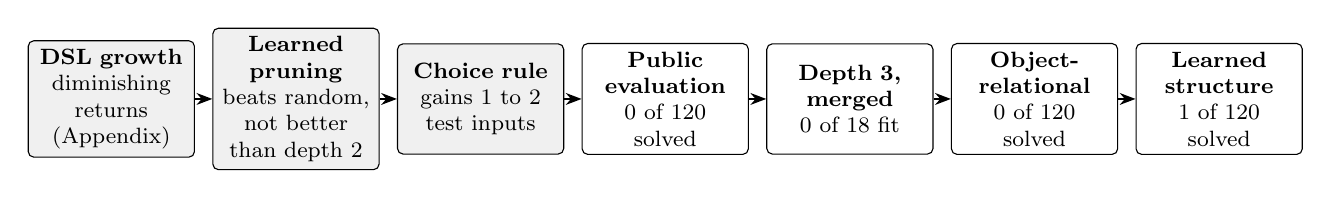
\begin{tikzpicture}[
  font=\footnotesize,
  box/.style={draw, rounded corners=2pt, align=center, inner sep=3pt, text width=19mm, minimum height=14mm, fill=white},
  good/.style={box, fill=black!6},
  arr/.style={-{Stealth[length=2mm]}, thick},
  node distance=3mm and 2.2mm]
  \node[good] (a) {\textbf{DSL growth}\\diminishing returns (Appendix)};
  \node[good, right=of a] (b) {\textbf{Learned pruning}\\beats random, not better than depth 2};
  \node[good, right=of b] (c) {\textbf{Choice rule}\\gains 1 to 2 test inputs};
  \node[box, right=of c] (d) {\textbf{Public evaluation}\\0 of 120 solved};
  \node[box, right=of d] (e) {\textbf{Depth 3, merged}\\0 of 18 fit};
  \node[box, right=of e] (f) {\textbf{Object-relational}\\0 of 120 solved};
  \node[box, right=of f] (g) {\textbf{Learned structure}\\1 of 120 solved};
  \draw[arr] (a) -- (b);
  \draw[arr] (b) -- (c);
  \draw[arr] (c) -- (d);
  \draw[arr] (d) -- (e);
  \draw[arr] (e) -- (f);
  \draw[arr] (f) -- (g);
\end{tikzpicture}
\Description{A row of six boxes joined by arrows. The first three, shaded, summarise the training-sample results: DSL growth, learned pruning and the choice rule. The last three summarise the public evaluation results: zero solved, no fit at depth 3 on 18 tasks, and zero for the object-relational solver.}
\caption{The chain of evidence. The three shaded boxes (left) are results on a fixed training sample, reported in the appendix, which show where the method gains and where it does not. The other four are results on public evaluation tasks: the first three show why the set stays at zero for the menu-based solvers, and the last shows the one solve of a rule-structure learner.}
\label{fig:chain}
\end{figure*}

\paragraph{Evidence tiers.} The flat-library ladder, the proposer comparisons and the choice-rule test are the clean, pre-specified experiments and are the primary evidence. The object-relational extensions and the cell-tree variants were developed on separate tasks but chosen and combined after seeing sample results, so they are secondary, exploratory evidence. The qualitative discovery, that learning the rule structure per task breaks the zero evaluation count of the fixed-menu solvers, rests on one public evaluation task; we claim only that changing the level at which hypotheses are built can break that zero, not that the method solves ARC-AGI-2.

\paragraph{Contributions.} The main ones are (a) a controlled decomposition of a symbolic ARC baseline into representation, search and selection, which shows that, within the tested regime, a larger DSL, learned pruning and better selection did not overcome the limited hypothesis space; (b) a test of learned search guidance, in which a task-conditioned proposer clearly beats random pruning at matched budgets but not exhaustive shallow search; and (c) a task-conditioned rule-structure learner that gives the study's only public-evaluation solve and a combined solver, with a cross-validation check that separates its correct fits from spurious ones. In more detail: (i) A complete, small, reproducible baseline for ARC-AGI-2 with numbers on both public sets; the code, trained proposers, task subsets and seeds accompany the paper as an archive. (ii) A controlled study of learned pruning and library growth on identical task subsets, with paired significance tests, five random seeds for the random control, and a proposer trained without the input grids of the test sample. (iii) A direct test of the choice rule against random choice among fitting programs. (iv) A set of diagnostic experiments that localise the method's failure modes and delimit what the tested symbolic representation can and cannot explain. (v) A search-redundancy audit and a merged-state search that make exhaustive depth 3 affordable for the first time in this setting. (vi) Three extensions of an object-relational solver and a rule-structure learner, with the negative and positive results reported for each, and a combined solver that is the basis of a Kaggle submission script.

We want to be plain about scope. The combined solver is a deliberately lightweight baseline, not a competitive system, and it was not developed on the hidden leaderboard test set. Its purpose is to make the experimental claims reproducible and measurable. The frozen solver was submitted once to the ARC Prize 2026 ARC-AGI-2 Kaggle competition and scored 1.67 on the hidden test tasks (Section~\ref{sec:kaggle}).

%% ==================================================================
\section{Background and Related Work}

\paragraph{The benchmark.} ARC was introduced together with an argument that intelligence should be measured by efficient skill acquisition on new tasks~\cite{chollet2019measure}. ConceptARC adds simpler tasks organised around single concepts to test whether systems really grasp them~\cite{moskvichev2023conceptarc}. A study of people solving ARC tasks describes human solving as program induction, which is one motivation for program-based methods~\cite{johnson2021fast}. ARC-AGI-2 keeps the format and adds a new, harder task set, with human testing as a baseline~\cite{chollet2025arcagi2}. The ARC Prize 2024 report names deep-learning-guided program synthesis and test-time training as the techniques behind that year's gains~\cite{chollet2024arcprize}.

\paragraph{Search over a DSL.} The strongest classical solutions enumerate programs in a hand-built DSL. The 2020 Kaggle winner is the best known~\cite{wind2020arcsolution}; its public README describes a search whose default depth is 2 and which can be set to depth 3. Hodel writes generators, expressed in a DSL of grid functions, that produce unlimited extra examples for ARC tasks~\cite{hodel2024rearc}. Our baseline is in this family. It is much smaller, and we study it with ablations rather than trying to maximise the score.

\paragraph{Learning to guide the search.} DeepCoder trains a network to predict properties of a program, such as which functions it uses, from its input-output examples, and uses these predictions to steer the search~\cite{balog2016deepcoder}. DreamCoder learns new library functions from solved tasks, together with a recognition network that guides search~\cite{ellis2020dreamcoder}. Our proposer follows the DeepCoder idea, with hand-made features rather than a learned encoder. We ask how far it carries on ARC-AGI-2.

\paragraph{Language models.} Recent work uses language models to write programs or to propose hypotheses and then checks them~\cite{wang2023hypothesis,butt2024codeit}. Object-based descriptions of the grid help language models a lot~\cite{xu2023llmarc}. Test-time training, where a model is updated on the examples of the task at hand, gave large gains on ARC-style tasks~\cite{akyurek2024ttt}. We use none of this. These methods need more compute than the two-core setting we work in, and we wanted a baseline whose every decision can be inspected.

\paragraph{Recent results on ARC-AGI-2.} The ARC Prize 2025 report says the best Kaggle entry reached 24\% on the private ARC-AGI-2 set, and names per-task refinement loops as the defining trend of the year~\cite{chollet2025prize2025}. Examples are evolutionary program synthesis, where a language model samples and refines programs and is fine-tuned on its own search attempts~\cite{pourcel2025soar}, and small networks trained or recursed at test time, such as a 7-million-parameter recursive model reporting 8\% on ARC-AGI-2~\cite{jolicoeur2025trm} and a 76-thousand-parameter model that minimises description length on the single target puzzle~\cite{liao2025compressarc}. Our system is far below competitive systems, and we do not compare numbers directly, because those reports use a different score (average over test inputs on the private set). The difference is one of purpose as much as of strength. Those systems are competitive solving architectures; ours is a controlled ablation of one symbolic mechanism. It uses no pretraining on ARC-like data beyond a small synthetic set, no test-time learning, and a fixed hand-written library, so we can change one factor at a time and measure it.

What the competitive systems share is that something is fitted to each task at test time: network weights, a refined answer, or a program. Our flat solver is the exception, since its hypothesis space is fixed before the task is seen. The cell-tree learner is a symbolic analogue of per-task fitting, with the structure of the rule, not a set of weights, learned from the examples. We therefore read our result as consistent with, not opposed to, the trend of the 2025 competition, and we do not claim that symbolic learning of this kind can match the neural systems.

\paragraph{Choosing among explanations.} When many programs fit the examples, something must pick one. We use an MDL-inspired length cost, based on the minimum description length idea of preferring the shortest explanation of the data~\cite{rissanen1978mdl,grunwald2007mdl}. Our version is a crude proxy, a program length plus a small charge for the colour map, and not a proper code length. It is a single number per program, so it is cheap and easy to check.

%% ==================================================================
\section{Problem Setup}

A task has a list of training pairs (usually two to five, at most ten) and one or more test inputs. A grid is a rectangle of whole numbers from 0 to 9 with each side at most 30. A prediction is correct only if it matches the true output exactly, cell by cell. ARC-AGI-2 allows two guesses per test input, and a test input counts as solved if either guess is exact. The score of a task is the share of its test inputs that are solved, and the score of a set is the mean over its tasks. We also report the number of tasks \emph{fully solved}, meaning every test input was solved. The two measures are nearly the same here because most tasks have one test input.

We use the public ARC-AGI-2 files~\cite{arcprize2025data}: 1{,}000 training tasks (1{,}076 test inputs, 69 tasks with more than one) and 120 public evaluation tasks (167 test inputs, 45 tasks with more than one). The public evaluation tasks are meant to be close in difficulty to the hidden leaderboard test set, while the training tasks are easier~\cite{chollet2025arcagi2}.

\paragraph{Terminology.} We call the two public sets \emph{training tasks} and \emph{public evaluation tasks}. We never used the hidden leaderboard test set for development; it was used once, for the Kaggle submission of Section~\ref{sec:kaggle}. A \emph{test input} is the input inside a task whose output must be predicted. A program \emph{fits} a task if it reproduces every training pair exactly (after one colour map). A fitting program is \emph{test-correct} if it also gives the true output on the test input; we avoid speaking of ``the right program'' because many different programs often fit. We say a search space has \emph{coverage} of a task if it contains at least one program, within the stated DSL, depth limit and colour-map mechanism, that fits the task. When we say that coverage is limited we mean this operational notion, and nothing about programs outside the searched space.

%% ==================================================================
\section{Method}

Figure~\ref{fig:pipeline} shows the whole pipeline. Every step is simple on purpose.

\begin{figure*}[t]
\centering
\resizebox{\textwidth}{!}{%
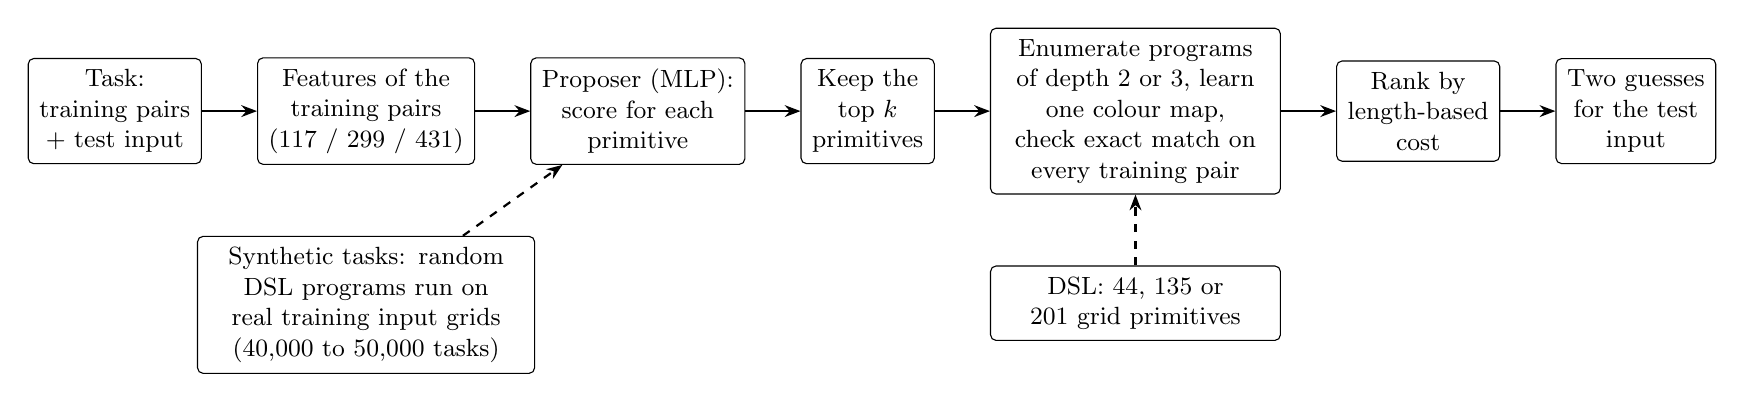
\begin{tikzpicture}[
  font=\small,
  box/.style={draw, rounded corners=2pt, align=center, inner sep=4pt, minimum height=9mm, fill=white},
  arr/.style={-{Stealth[length=2mm]}, thick},
  darr/.style={-{Stealth[length=2mm]}, thick, dashed},
  node distance=5mm and 7mm]
  \node[box] (task) {Task:\\training pairs\\+ test input};
  \node[box, right=of task] (feat) {Features of the\\training pairs\\(117 / 299 / 431)};
  \node[box, right=of feat] (prop) {Proposer (MLP):\\score for each\\primitive};
  \node[box, right=of prop] (topk) {Keep the\\top $k$\\primitives};
  \node[box, right=of topk, text width=34mm] (search) {Enumerate programs of depth 2 or 3, learn one colour map, check exact match on every training pair};
  \node[box, right=of search] (mdl) {Rank by\\length-based\\cost};
  \node[box, right=of mdl] (out) {Two guesses\\for the test\\input};
  \draw[arr] (task) -- (feat);
  \draw[arr] (feat) -- (prop);
  \draw[arr] (prop) -- (topk);
  \draw[arr] (topk) -- (search);
  \draw[arr] (search) -- (mdl);
  \draw[arr] (mdl) -- (out);
  \node[box, below=9mm of feat, text width=40mm] (syn) {Synthetic tasks: random DSL programs run on real training input grids (40{,}000 to 50{,}000 tasks)};
  \draw[darr] (syn) -- (prop);
  \node[box, below=9mm of search, text width=34mm] (dsl) {DSL: 44, 135 or 201 grid primitives};
  \draw[darr] (dsl) -- (search);
\end{tikzpicture}}
\Description{A flow chart. A task goes through feature extraction, a proposer network that scores each primitive, selection of the top k primitives, program enumeration with exact checking, ranking by description length, and two guesses. Synthetic tasks train the proposer once and the DSL feeds the enumeration step.}
\caption{The pipeline. Solid arrows run for every task. Dashed arrows are set up once: the proposer is trained once on synthetic tasks, and the DSL is fixed beforehand.}
\label{fig:pipeline}
\end{figure*}

\subsection{Grids and objects}

The background colour of a grid is its most frequent colour. An \emph{object} is a group of touching non-background cells, where touching includes diagonals. Some primitives use objects of one colour only; others allow mixed colours. Everything else in the DSL works directly on the grid.

\subsection{The DSL in three sizes}

A primitive takes one grid and returns one grid, or returns nothing when it does not apply (for example, ``crop to the largest object'' on an empty grid). Primitives never use a fixed colour. When a primitive needs a new colour it takes the first colour from 1 to 9 that is not in the grid, and the colour map described below turns it into the real colour. We built the DSL in three tiers so that the effect of each step can be measured. Table~\ref{tab:dsl} lists them.

\begin{table}[t]
\caption{The three DSL tiers. Each tier contains the previous one.}
\label{tab:dsl}
\small
\begin{tabular}{@{}p{0.6cm}p{0.9cm}p{5.2cm}@{}}
\toprule
Size & New & What the new primitives do \\
\midrule
44 & 44 & Rotations and flips (7); crop to an object, drop noise (8); scale, tile, mirror (9); halves of the grid (4); gravity in four directions (4); fill holes, symmetry, outline, extend lines, remove repeated rows, colour summaries, overlay halves (12) \\
135 & 91 & Pick or drop a colour by rank (9); recolour or select objects by size, holes, border contact (9); drop, shift or roll the grid (12); draw lines and join pixels (9); borders and fills (5); and, or, xor, nor of halves (8); pick a cell of a grid of cells (4); more tiling and joining (14); counts (3); dilate, erode, denoise (4); complete symmetry (2); sort (2); swap and binarise colours (3); thirds (4); per-object flip and box (3) \\
201 & 66 & Conditional object rules: 14 tests (largest, smallest, touches border, inside, has hole, filled rectangle, single cell, above mean size, taller than wide, unique shape, repeated shape, most common colour, rarest colour, mirror symmetric) times 5 actions (recolour, remove, keep only, fill box, flip), minus 4 pairs that can never change a grid \\
\bottomrule
\end{tabular}
\end{table}

\subsection{Program search with exact checking}

A \emph{program} is a list of primitives, applied one after the other, followed by an optional colour map. We search all programs up to a depth limit $d$. For each training pair we run the program on the input. The program is \emph{consistent} if its result equals the expected output on every pair, after one colour map shared by all pairs.

\emph{Colour map, formally.} Let $p(x)$ be the grid a program produces from input $x$. A colour map $m$ is a function from colours to colours, applied to every cell. It is total on the colours that occur in some $p(x_i)$ and the identity on every other colour. A program is consistent with training pairs $(x_1,y_1),\dots,(x_n,y_n)$ if there is one map $m$ with $m(p(x_i))=y_i$ for every $i$. We do not search for $m$; we read it off. The program output must have the same size as $y_i$ on every pair. Every colour $c$ that occurs in some $p(x_i)$ is then constrained by at least one output cell: all output cells $y_i$ at positions where $p(x_i)$ has colour $c$ must show the same colour, and that colour is $m(c)$. So no colour that occurs in a program output is ever left without a value. If two different colours would be needed, the program is rejected. The map may merge colours (many-to-one), and colours that never occur in the training program outputs map to themselves, so a test input may contain colours that $m$ does not mention. A map that changes nothing is dropped. Because $m$ is read off and not searched, it adds no branching to the search.

\emph{Failures and limits.} If a primitive raises an error or returns a grid with a side outside 1 to 30, it counts as returning nothing and the prefix is dropped. Every loop in the DSL is bounded by the size of the grid, so no timeouts were needed.

Search is breadth first. The grids that a prefix produces are stored, so a prefix is computed once for all programs that share it. If a primitive returns nothing on any training input, that prefix is dropped. With $n$ primitives, depth 2 means about $n^2$ programs: roughly 1{,}900 for 44 primitives, 18{,}000 for 135 and 40{,}000 for 201. Depth 3 over all primitives is out of reach for the larger tiers in routine runs (about 2.5 million programs for 135 and 8 million for 201), which is where pruning is supposed to help. Time per primitive application, measured over the runs below, is about 50 microseconds for the 44 tier and 75 to 90 microseconds for the larger tiers, so cost grows mainly with the number of programs.

\subsection{Choosing among consistent programs}

Many programs can fit the same examples. We give each a length-based cost: the number of primitives, plus 0.25 for every colour in the map that changes colour. We chose the 0.25 in advance and did not tune it, and Section~\ref{S-sec:sel} tests only whether this MDL-inspired length cost beats random choice, not whether 0.25 is a good weight. The cheapest program wins, and ties are broken by the order in which programs were found (shorter programs first, then DSL order). The first two programs with different results on the test input give the two guesses. If only one distinct result exists, the second guess repeats the first.

\subsection{A learned primitive proposer}

\paragraph{Features.} For each training pair we compute 29 numbers about how the output relates to the input: size ratios, whether the shape stays the same, whether the output is a whole multiple or fraction of the input, colour counts, how many cells change, left-right and up-down symmetry, whether the output appears inside the input, and object counts. We then add two numbers for every primitive: whether its result has the right shape, and what fraction of cells already match the output. We average over the training pairs of the task. This gives $29+2n$ numbers: 117, 299 or 431 for the three tiers.

\paragraph{Synthetic training tasks.} We build tasks for which the answer is known. We draw a random program of depth 1, 2 or 3 (with probability 0.45, 0.35, 0.20), choosing primitives uniformly. With probability 0.15 we also apply a random colour permutation. We take three input grids at random from the input grids of public training tasks, run the program, and keep the task only if no output equals its input. The label is the set of primitives used, plus one flag for ``a colour map was needed''. Only input grids are used, never the public outputs, and the evaluation set is never touched. We trained two versions of the proposer for the 135 and 201 tiers. The \emph{original} proposer draws grids from all 1{,}000 training tasks, so it has seen the inputs (never the outputs) of the 300 sampled tasks. The \emph{disjoint} proposer draws grids only from the 700 training tasks outside the 300-task sample, so it has seen no grid from a sampled task. We made 40{,}000 tasks for the 44-primitive proposer, 50{,}000 for each original proposer of the larger tiers, and 40{,}000 and 50{,}000 for the disjoint proposers of the 135 and 201 tiers. The 44-primitive proposer exists only in the original version.

\paragraph{Model.} A two-layer network (256 and 128 units) trained with Adam~\cite{kingma2015adam} in scikit-learn~\cite{pedregosa2011sklearn}, with one output per primitive, early stopping and at most 60 passes. We hold out 10\% of the synthetic tasks to measure \emph{recall at $k$}: the share of tasks for which every primitive of the true program is among the $k$ highest-scored ones. This measures how well the proposer learned the generator. It is not the same as how well it helps on real tasks. Because several primitive sequences can be semantically equivalent, the metric may also understate useful pruning. We therefore treat downstream task solving as the primary measure of the proposer, and add a solution-preserving recall on real tasks in Section~\ref{S-sec:recall}.

\subsection{Guided search and the random control}

In guided search we compute the features of a task, keep the $k$ highest-scored primitives, and enumerate programs only over them (the colour map is always available). We use $k$ of 16, 24 and 32, picked by hand. The value $k=16$ was the initial setting; $k=24$ and $32$ were added during development, after training-set results showed that the smaller values lost tasks. We therefore treat $k=16$ as the pre-specified setting and the larger values as exploratory. As a control, \emph{random pruning} keeps $k$ primitives chosen uniformly at random for each task, with the seed set from the task name. This control tells us how much of any gain comes from the proposer's knowledge and not just from searching less. We repeat it with five seeds. Guided and random runs with the same $k$ keep the same number of primitives, which we call the same \emph{pruning budget}. The random control was run at $k=16$ for the 44 library and at $k=24$ for the larger ones, so only the $k=24$ guided runs have a random control at the same budget. The search itself then costs about the same, but not exactly, because programs differ in how many survive the early checks, so we report both seconds and search nodes (primitive applications to training grids).

\subsection{Learning the rule structure}
\label{sec:cell}

The solvers above choose from a fixed menu. As a first step toward learning the structure of a rule from the examples, we built a solver for same-size tasks in which the rule is a small decision tree over per-cell features. For every cell it computes colour-valued features (its own colour, the eight neighbours, the nearest coloured cell along each of eight rays, mirrored cells, the nearest coloured cell in any direction, and the colour that surrounds an enclosed background region), numeric features (row and column, parities, ray distances, neighbour counts, the size of the cell's object, whether the object touches the border or has a hole or is the largest or smallest, and whether a background cell is enclosed), and tests built from them. It also lists candidate \emph{sources} for the output colour: the cell's own colour, a constant, a neighbour, a ray colour, a mirrored cell, the most or least common colour, and the colour of the largest or smallest object. A leaf of the tree may use a source only if that source gives the correct output colour for every training cell that reaches the leaf, so a leaf is a rule such as ``copy the colour of the nearest coloured cell above''.

The tree is grown greedily. At each node the solver picks the test after which the two children are best covered by single sources, and it deepens the tree one level at a time up to depth 5, so smaller trees are preferred. It fits four variants of the feature set (with and without position features, with and without ray features), checks each by exact reproduction of every training output, and ranks the surviving trees by \emph{leave-one-pair-out} reproduction (a tree fitted to all pairs but one must reproduce the held-out pair), then by tree size. The tests, their order and the leaves are learned for each task, in contrast with a menu. The solver handles same-size tasks only, has no notion of moving or copying whole objects, and can only produce colours from the sources it lists.

%% ==================================================================
\section{Experimental Setup}

\paragraph{Subsets and compute.}\label{sec:setup-note} Everything ran on two CPU cores with no GPU (Python 3.13, NumPy~\cite{harris2020numpy}, SciPy~\cite{virtanen2020scipy}, scikit-learn). Unpruned search is slow for the larger tiers, so the main comparison uses one fixed sample of 300 of the 1{,}000 training tasks (321 test inputs), drawn with a fixed random seed (20261014) and shared by every setting. Every row of Table~\ref{S-tab:main} is measured on exactly these tasks, on the same machine, so times and counts are directly comparable. This sample has 89 tasks in common with the first 300 tasks in alphabetical order, which our first runs used. We dropped that subset because alphabetical order is not a random sample, and it gave higher solved counts than the random sample does. The 44-primitive tier was also run on all 1{,}000 training tasks (Section~\ref{S-sec:small}). All settings were run on all 120 public evaluation tasks. The depth-3 diagnostic of Section~\ref{sec:dedup} used 18 of them, drawn at random in two batches of 2 and 16. \emph{Seconds per task} is the mean wall-clock time per task, including feature extraction for guided runs. \emph{Nodes} counts primitive applications to training grids made by the search, in thousands; it does not depend on the machine.

\paragraph{Sanity checks.} All 120 evaluation tasks and their 167 test inputs have the true outputs in the public files and no malformed grids (every grid is two-dimensional with values 0 to 9), so a score of zero cannot come from missing answers. The same scoring code gives non-zero scores on training tasks and reproduces three of the solved examples of Table~\ref{S-tab:examples} (1e0a9b12, 1b2d62fb, 3618c87e).

\paragraph{Search redundancy.} The main solver caches prefix results but does not merge programs that give the same grids. We measured how much work this wastes on the 201 library: on three sample tasks, depth-2 programs (12{,}971 to 15{,}408) reach only 19\% to 40\% distinct final states, and at depth 1, 2{,}705 programs over 20 tasks give 1{,}964 distinct states (73\%). The node counts we report therefore include a large amount of redundant work, and a search that merges equal states is several times cheaper at depth 3 (Section~\ref{sec:dedup}).

\paragraph{Statistics.} Intervals are 95\% Wilson score intervals~\cite{wilson1927interval}. To compare two settings on the same tasks we count the tasks that only one of them solves and apply an exact two-sided sign test to those counts. We designated two families as \emph{primary}, after the experiments were run and from the study's questions, so the designation is not pre-registered: the two library-growth comparisons (44 to 135, 135 to 201), and the proposer-versus-random comparison. The latter consists of 10 matched paired comparisons: for each of the five random seeds and each of the 135 and 201 libraries, the (deterministic) disjoint proposer at $k=24$ is compared task by task with the random control at $k=24$. Every other test (about 25 more) is exploratory, is reported without correction, and a single $p$ between 0.01 and 0.05 among them should be read as weak evidence. For the proposer at $k=32$ we also computed 10 comparisons, but the random control keeps only 24 primitives, so these are not at a matched budget; we do not count them as primary and only note that they point the same way.
\paragraph{Evaluation discipline.} We did not inspect individual public evaluation tasks during development. No design choice was made using results on individual evaluation tasks. The solvers of Sections~\ref{S-sec:orelx} and \ref{S-sec:celltree} were developed on the 700 training tasks outside the 300-task sample, frozen, and run once on the sample and once on the evaluation set; we did not look at any evaluation task before those runs. The choice to put the last object-relational variant into the combined solver was made after seeing sample results (it is a superset of the earlier ones), so it is exploratory. Choices were of two kinds. \emph{Pre-specified:} the primitives of the 44 tier, the cost weight 0.25, the generator settings, $k=16$, the 300-task sample and the number of seeds. \emph{Exploratory, driven by training-set results:} the larger values of $k$ (24 and 32), the DSL tiers beyond 44, and the actions of the object-relational solver (adjusted only on tasks outside the 300-task sample). The random 300-task sample, the seeds and the experiments described here were fixed after an external review of an earlier draft and are not a response to the sample's results.

%% ==================================================================
\section{Results}

This section reports the public evaluation set, which is the set the Paper Prize asks for. Experiments on a fixed sample of public training tasks, which support the diagnosis but are not evaluation scores, are in Supplement~\ref{S-app:train}.

\subsection{Kaggle submission}\label{sec:kaggle}

We submitted the combined solver (flat DSL with 201 primitives, then \texttt{orel5}, then \texttt{celltree2}), frozen, as a CPU-only Kaggle notebook with internet disabled and no pretrained model. One run on the 240 hidden test tasks scored 1.67, which is 4 of 240 tasks if every task counts equally. That is above the 1 of 120 (0.8\%) on the public evaluation set (Table~\ref{tab:evalsum}), but the task sets differ and are small, so we do not read the gap as an improvement. A run on the placeholder test file took 3{,}141 s on four processes. The scored notebook is Version 2 at \url{https://www.kaggle.com/code/joyboseroy/notebookf09093f843?scriptVersionId=362153283}; the code is released under the MIT-0 licence, and the runner (\texttt{kaggle\_run.py}) accompanies the paper.

\subsection{The public evaluation set}

\subsubsection{No fitting program at depth 2}\label{sec:eval}

We ran thirteen settings on all 120 public evaluation tasks (167 test inputs); a setting here is one search configuration on one library with the original proposer where a proposer is used, and one random seed. For the 44 library: plain depth 2, proposer top-16 at depth 2, top-16 and top-24 at depth 3, random-16 at depth 3 (five settings). For each of the 135 and 201 libraries: plain depth 2, proposer top-24 and top-32 at depth 3, random-24 at depth 3 (four settings each). The disjoint proposers, the extra random seeds and the extra proposer seeds were not run on the evaluation set. None of the thirteen settings solves any of the 120 public evaluation tasks. The 95\% upper bound on the true solved share of tasks is about 3.0\%. More telling: in every one of these runs, the number of evaluation tasks for which the search found \emph{any} program that fits the training pairs is zero. Wrong choices among fitting programs therefore cannot be the cause. All of those runs searched depth 2 over all primitives, or depth 3 over the top-$k$ primitives. To test whether depth 3 over all primitives changes this, we ran exhaustive depth-3 search on a random sample of evaluation tasks: all 44 primitives on 12 tasks (a tenth of the set) found no fitting program for any of them, and a search with 201 primitives that merges equal states (Section~\ref{sec:dedup}) found none on 18 evaluation tasks (15\% of the set). These are samples, so they limit but do not exclude fitting programs at depth 3 on the rest of the set, and they say nothing about depth 4 or more.

\subsubsection{How close does the search get?}

\input{diag_text}

\begin{table}[t]
\caption{Diagnostic with the 201-primitive library, programs of depth up to 2, no colour map. Columns: the random 300 training tasks split by whether plain depth-2 search solved them, and the 120 evaluation tasks. Same size: output has the input's size. Shape ok: some program has the right output size on every training pair. Best match: median over those tasks of the best share of matching cells (all cells, or only cells that are not background in the target or the prediction). Copy match: the same for copying the input, on same-size tasks. Gain $>5$: same-size tasks where the best program beats copying by more than five points.}
\label{tab:diag}
\footnotesize\setlength{\tabcolsep}{4pt}
\input{diag_table}
\end{table}

\subsubsection{Does the solve rate depend on task size?}

The evaluation grids are larger than the training grids (Table~\ref{tab:diag}), so a drop in solve rate is expected even for a method that is otherwise the same. In the training sample the solve rate of the flat solver falls steeply with grid size, and the public evaluation tasks lie in a harder region of the size range (Supplement~\ref{S-sec:size}). Size is probably a proxy for structural complexity and not itself an explanation: a large grid with two objects can be easier than a small grid with a complicated relational rule.



\subsubsection{Is depth the limit? Exhaustive depth 3 with merged states}
\label{sec:dedup}

The main solver treats programs that give the same grids as different programs. Because many primitives overlap, this wastes most of the work at depth 2 (see the redundancy audit in Section~\ref{sec:setup-note}). We wrote a second search that asks only whether a fitting program of depth up to 3 exists. It expands each distinct state, meaning the tuple of grids a program produces on all training inputs, only once, and checks every one-step extension for a fit with one global colour map. It cannot tell which of several equivalent programs is best, so it answers existence, not accuracy.

With 201 primitives the merged search is much cheaper than the full one: a task has about 9{,}500 to 10{,}800 distinct states after two steps, against about 40{,}000 depth-2 programs and 8 million depth-3 programs, and one task needs about 5.7 million primitive applications and about 15 minutes (the slowest 105 minutes, for large grids). We ran it on 18 randomly selected public evaluation tasks (15\% of the set; the draw was made in two batches of 2 and 16 tasks). \textbf{No task has a fitting program of depth up to 3.} Together with the depth-2 result on all 120 tasks, this gives no evidence that a missing third step alone explains the zero on the sampled public evaluation tasks, and deeper programs remain untested. This makes a systems point. Depth 3 can add coverage on training tasks (Supplement), the cost of enumerating programs is large, and fixed-$k$ pruning can miss exactly the tasks it would unlock. What the audit shows is that the cost depends on the number of distinct states, not on the number of programs, which suggests searching over states.

The result is limited in three ways. It covers 18 of the 120 tasks and depth up to 3, not deeper programs. It uses the 201 primitives, so a task that needs a missing concept would not be found at any depth. And it uses a single global colour map. We therefore claim only that, for these 18 tasks, adding a third step to the existing library does not produce a fitting program.

\subsubsection{Does a limited object-relational solver help?}
\label{sec:orel}

An obvious objection to this whole study is that its hypothesis language is flat (Section~\ref{sec:disc}). We therefore built a second, limited object-relational solver with a richer language and compared it with the flat one on the same tasks. It is a first version and does not represent the whole family of object-centric ARC systems; from here on we call it the object-relational solver. It handles tasks whose output has the input's size (204 of the 300 sample tasks and 81 of the 120 evaluation tasks) and works in four steps.
\begin{enumerate}
  \item \emph{Objects.} The grid is split into objects in three ways: same-colour 8-connected, same-colour 4-connected, and multicolour 8-connected components.
  \item \emph{Correspondence by labelling.} Each input object is labelled with every action that reproduces the output around it: keep, remove, recolour to a constant or to the colour of a related object (nearest, touching, container, largest, smallest, same shape), fill its box or holes, move by a vector, slide until blocked, flip, outline, draw a ray in eight directions, draw a line or frame, or connect to objects in the same row or column. There are 234 such actions. Changed background cells count as changes that some object's action must explain.
  \item \emph{Rule induction.} The solver searches for the shortest decision list of at most four rules. Each rule is one or two literals (an object property such as largest, hole, border; or a relation such as touching, inside, aligned, or same shape as some object, optionally with the other object's colour) and one action, and a rule may only fire on objects for which its action is consistent. A greedy cover picks the rules.
  \item \emph{Exact check.} The decision list is rendered on every training pair and must reproduce each output exactly. The cost of a rule set is its number of rules plus literals, and up to two predictions come from the cheapest rule sets over the three object definitions.
\end{enumerate}
To keep the comparison clean, we developed this solver only on the 700 training tasks outside the 300-task sample, over four rounds in which we added action types after looking at aggregate failure counts. It solved 20, 25 and then 28 of the 700 (4.0\%) in the last rounds. We then froze it and ran it once on the sample and once on the evaluation set. The flat solver was not changed. The object-relational experiment is therefore a frozen exploratory extension, not a pre-registered comparison.



On the 120 public evaluation tasks the new solver solves none and finds a fitting rule set for only one task (97d7923e), which is wrong on the test input. It takes 3.3 s per task. So the richer language does not unlock the evaluation set (its comparison with the flat solver on the training sample is in the Supplement). This is evidence against the simplest version of the objection, that object properties, one-step relations to other objects, and conditional actions are what the flat solver lacks. It does not refute the broader one: our rules have no variables, no iteration, no multi-step composition of actions and no object correspondence beyond in-place labels, and the solver covers only same-size tasks. This experiment rejects only the narrow hypothesis that adding our particular set of object properties, one-step relations and conditional actions is enough to recover the public evaluation tasks. The comparison is therefore between two incomplete languages, a flat chain of whole-grid operations and a fixed menu of object rules, and not between a flat language and a complete object-centric one.


%% ==================================================================
\subsection{Learning the rule structure on the evaluation set}
\label{sec:evalcell}

The rule-structure learner of Section~\ref{S-sec:celltree} is the only solver in this study that solves a public evaluation task. Table~\ref{tab:evalsum} summarises every solver we ran on the 120 tasks. Each solver was developed on training tasks outside the sample, frozen, and run once on the evaluation set; we did not inspect any evaluation task before those runs. The cell trees solve task aa4ec2a5 and find fits for five further tasks, all wrong. The three extensions (a primitive before the tree, block features, and colour canonicalisation or augmentation, Supplement~\ref{S-app:train}) change the number of fits, from 1 to 9, but every one solves the same single task and no other. The combined solver (flat, object-relational and residual cell trees) also solves 1 of 120 (0.8\%; 95\% interval 0.1 to 4.6) at 27.5 s per task. The solve rate of the cell trees falls with grid size on development tasks (Supplement~\ref{S-app:train}), and public evaluation grids are larger on average, which is one plausible reason why training gains do not transfer; we did not test that further.

\begin{table}[t]
\caption{All solvers on the 120 public evaluation tasks. Fits: tasks for which a program or rule fitting every training pair was found.}
\label{tab:evalsum}
\footnotesize\setlength{\tabcolsep}{4pt}
\begin{tabular}{@{}>{\raggedright\arraybackslash}p{3.6cm}rr@{}}
\toprule
Solver & Solved & Fits \\
\midrule
Flat DSL (13 settings) & 0 & 0 \\
Object-relational (4 variants) & 0 & 1 \\
Cell trees & 1 & 6 \\
Cell trees 2 (primitive first) & 1 & 7 \\
Cell trees 4 (block features) & 1 & 9 \\
Colour-canonical trees & 1 & 7 \\
Augmented trees & 1 & 1 \\
Object trees (two action menus) & 0 & 2 \\
Combined solver & 1 & \\
\bottomrule
\end{tabular}
\end{table}

\paragraph{Object trees.} A natural next step was a tree over object and relation features that chooses object actions, combining the object-level and the structure-learning solvers. We built it: the objects, relations and actions are those of the object-relational solver (with its first and its last action menu), and the structure of the rule is a decision tree of depth up to four over object, rank, count and relation features instead of a decision list of at most four short rules. It was developed on the development tasks only, frozen and run once. It solves none of the 120 evaluation tasks and finds fits for two, both wrong. On the development tasks it solves fewer tasks than the decision-list solver it replaces (23 and 25 of 700 for the two menus, against 39), but its fits are more often right (23 of 39 and 25 of 41), and it adds only 3 tasks to the union of the object and cell-tree solvers (Supplement). So learning the structure of the object rule as a tree, with these features, does not by itself reach the evaluation tasks; the limit is more likely in the features and in the actions available than in the form of the rule.

The fits of the cell trees are spurious more often than those of the flat solver, but a leave-one-pair-out check separates them. On the development tasks, among fits for tasks with at least three pairs, those that reproduced every held-out pair were correct 20 times out of 21, against 15 of 79 for the others, and for none of the 90 wrong development fits was any other candidate tree correct. The failures are therefore failures of construction, not of ranking.

\section{Discussion}

\label{sec:disc-top}The experiments answer three questions, and they fail in three different ways. \emph{Representation}: does a fitting program exist in the searched space? \emph{Search}: can the search reach it affordably? \emph{Selection}: if several programs fit, can the correct one be picked? Table~\ref{tab:rss} maps each experiment to one of them.

\begin{table}[t]
\caption{Experiments mapped to the three questions.}
\label{tab:rss}
\footnotesize\setlength{\tabcolsep}{4pt}
\begin{tabular}{@{}>{\raggedright\arraybackslash}p{1.4cm}>{\raggedright\arraybackslash}p{3.0cm}>{\raggedright\arraybackslash}p{2.9cm}@{}}
\toprule
Question & Experiment & Result \\
\midrule
Representation & DSL 44, 135, 201 & large gain, then small \\
 & Object-relational solver & +7 training, 0 evaluation \\
 & Foreground diagnostic & best candidate about as close as copying \\
Search & Proposer against random & proposer better \\
 & Proposer against depth 2 & depth 2 better or tied \\
 & Merged depth 3 & 0 of 18 fit \\
Selection & Shortest-first against random & modest gain \\
\bottomrule
\end{tabular}
\end{table}

\paragraph{Within the tested search regime, coverage is a stronger limitation than selection.} When a fitting program is found it is test-correct about nine times out of ten: 19 of 21 tasks with a fitting program are solved with 44 primitives, 28 of 31 with 135 and 30 of 33 with 201 (the 44-primitive run on all 1{,}000 tasks gives 67 of 75). Choosing at random among fitting programs would lose at most one or two test inputs (Table~\ref{S-tab:sel}). On the public evaluation tasks no fitting program exists at depth 2. Together these results say that, in the regime we tested (mostly depth 2 over a flat library), the tested space contains too few fitting hypotheses, which is consistent with growing the library helping and a better choice rule adding little. The claim has an operational meaning: the depth-2 hypothesis space, with this DSL and this colour-map mechanism, has inadequate coverage. We have not shown that no program exists anywhere in the DSL. Programs of depth 3 or more, a different cost rule, or a differently built library might change the picture, and our depth-3 evidence on the public evaluation set is a sample.

\paragraph{Why the evaluation set stays at zero for the menu-based solvers.} The evidence points to four linked causes, in this order. (1) Representation: no depth-2 program in any of the three libraries fits the training pairs of any of the 120 evaluation tasks, and exhaustive merged-state search through depth 3 finds no fit on 18 of them, so there are no fitting programs for choice or search guidance to act on. (2) Size: the evaluation tasks have larger grids (mean output 290 cells, against 43 for solved and 158 for unsolved training tasks), and the solve rate of both the flat and the cell-tree solver falls with grid size. (3) Distance: the best depth-2 candidate on the evaluation tasks is slightly less close to the answer than copying the input (median foreground overlap 52.1\% against 54.5\%), so the failures are not near misses. (4) Expressiveness of our object menu: it has no variables, no multi-step rules chained on each other's output and no general correspondence across size changes, and extending it increased training coverage only. We did not test whether adding these would help, and the first of them is the direction we propose. We cannot separate size from rule difficulty, because larger grids tend to go with more complex rules.

\paragraph{Learning the structure helps where menus do not.} The rule-structure learner of Section~\ref{S-sec:celltree} solves tasks the flat solver misses and adds substantial coverage on training tasks (Supplement), whereas the extensions of the object menu added little. The difference suggests that the useful kind of coverage is not more menu items but a language in which the structure of a rule is learned from the examples. The learner has its own ceiling: it works per cell, cannot move or copy whole objects, and solves a single public evaluation task, so the evaluation gap is far from closed. It also fails differently from the object solver, which is why the two combine well.

\paragraph{Coverage and spurious fits trade off.} The experiments show a three-way tension. A small library or a rigid rule menu leaves tasks without any fitting program. A richer language such as the object-relational one gains coverage on training tasks but its fits are less reliable than those of the flat language (Supplement). Pruning cuts search cost, but it can lose the very primitives that a rare task needs. Too little representation gives no fit, and too much unconstrained representation gives spurious fits, so an expressive language needs a way to keep its explanations in check.

\paragraph{Search over states, not programs.} The redundancy audit shows that the work of the enumeration depends on the number of distinct states reached, not on the number of programs. That favours a different next system: a richer compositional language, merging of equal states, and a learned ordering of the search. We say this as a direction suggested by the audit and the depth-3 runs, not as a tested result.

\paragraph{What the representation cannot say.}\label{sec:disc} The strongest criticism of this design is that its hypothesis language is flat. A program is a chain of whole-grid operations with one global colour map. It has no variables, so it cannot say ``take the smallest object and move it to the largest one''. It has no explicit relations between objects (left of, inside, touching, aligned), no correspondence between input and output objects, and no general map, filter or branch over objects. The 66 conditional primitives are fixed pairs of one object test and one action. They are a menu, not rule induction, which may be why they added little. Section~\ref{sec:orel} tests a first version of this objection with an object-relational solver. It helps a little on training tasks and not at all on the evaluation tasks, so the objection is not supported in that form, though our rules are still far from variables, iteration and general correspondence. We list the experiments that would go further in Section~\ref{sec:next}.

\paragraph{Library expansion is not representation expansion.} The 44, 135 and 201 comparison should be read as a test of library expansion within a fixed representation, not as evidence that a sufficiently expressive DSL has been ruled out. Adding operators to a flat whole-grid language is different from adding objects, relations, variables and conditional composition to the language. Section~\ref{sec:orel} tests only a small step of the second kind.

\paragraph{Diminishing returns from hand-written primitives.} The first growth step gave 9 more solved tasks on the fixed 300, and the second gave 2. One possible reason is that many of the conditional rules are narrow variants of rules already in the 135 tier, though we did not test this. The diagnostic suggests that evaluation tasks need rules that depend on the task more than a fixed menu of test-and-action pairs can express.

\paragraph{When learned pruning is worth it.} The proposer clearly beats random pruning, so it learns useful primitive-level information under the synthetic task distribution, and this is not an artefact of having seen the input grids of the 300-task sample, since a proposer trained without them behaves the same. But at depth 2 over up to 201 primitives, brute force finishes in under 10 seconds per task on two cores, so there is little to save. Pruning pays off when the search is deep: over 44 primitives, top-24 pruning at depth 3 is several times faster than unpruned depth 3 at a small loss in solved tasks (Supplement). For larger libraries it did not keep enough at a fixed $k$. The main lesson is not that learned pruning fails. Learned pruning can move efficiently through a hypothesis space, but it cannot make up for a space that holds too few useful explanations.

\subsection{What the experiments establish}\label{sec:established}

\emph{Established, within the tested regime:} (i) on a fixed training sample, moving from 44 to 135 primitives increases the number of fully solved tasks and moving from 135 to 201 adds little (Supplement); (ii) learned pruning beats random pruning at a matched budget; (iii) at depth 2, with affordable cost, pruning does not beat unpruned search; (iv) fitting programs are usually test-correct; (v) shortest-first adds a modest benefit over random choice; (vi) no depth-2 program fits any of the 120 public evaluation tasks; (vii) no depth-3 program fits any of 18 sampled public evaluation tasks; (viii) three extensions of the object-relational menu add training coverage but no evaluation solves; (ix) a solver that learns the rule structure per task adds training coverage and one public evaluation solve, and its fits can be filtered by leave-one-pair-out reproduction; (x) letting the learner apply a primitive first doubles development coverage (50 to 98), and block features, colour canonicalisation and augmentation add little, yet none raises the evaluation count above 1 of 120, and the solve rate falls with grid size on training tasks.

\emph{Not established:} that no program of depth 4 or more exists; that no richer DSL can solve the public evaluation tasks; that object-centric reasoning is insufficient; that learned search is fundamentally unhelpful; that coverage is the main bottleneck for ARC-AGI-2 in general; or that one solved evaluation task predicts a useful evaluation score.

\paragraph{Threats to validity.}
\begin{itemize}
  \item The proposer is trained on random programs from the same DSL, not on programs for real tasks. It learns to recover the ingredients of a random program, which may differ from the distribution of rules that task designers use. Its features also include how well each single primitive already matches the output, which helps shallow programs but says little when no single step resembles the answer. We did not train on real solved tasks, test a proposer without the per-primitive features, or score pairs of primitives together.
  \item The proposer's features are global averages over training pairs. They cannot express spatial relations such as one object inside another or the distance between two objects. A model over objects or scene graphs could do better; we did not try one.
  \item The synthetic tasks reuse input grids from public training tasks. The disjoint proposers address this for the 300-task sample and give the same results, so we do not expect leakage to explain our findings. The solution-preserving recall of Section~\ref{S-sec:recall} is computed on real tasks; we did not compute a solution-preserving recall on synthetic tasks. Grids of real ARC tasks still shape the synthetic distribution, and we did not test fully procedural grids.
  \item The cost weight and the generator settings were fixed in advance and not tuned, while the larger values of $k$ were added after early training-set results and are exploratory. Other choices could change the numbers.
  \item The cell-tree solver and the later object-relational variants were developed over two to four rounds on the 700 development tasks, and the sample was used to choose which object-relational variant enters the combined solver. Its training-sample results are therefore less clean than the flat-library numbers, though the sample was never used to tune any solver. The evaluation set was run once per frozen solver.
  \item The 300-task sample is random but small. Its intervals are wide (for example 7.1\% to 13.9\% for 201 primitives), and the earlier alphabetical sample gave clearly higher numbers. Differences of a few tasks are within noise, and we lean on paired tests, which are exact but have little power at these sizes.
  \item The random baseline uses five seeds. Proposer training noise was measured for top-24 depth 3 only (three seeds, Section~\ref{S-sec:recall}), and the spread for the 201 library is 24 to 30 solved tasks. The random control was not run at $k=32$, so the $k=32$ comparisons with random pruning are not at a matched budget.
  \item One author, one machine. Solved counts are deterministic given the seeds in the scripts, but timings depend on the machine, which is why we also report search nodes.
\end{itemize}

\paragraph{Limitations.} We did not use a language model or test-time training, both of which are known to help on ARC tasks~\cite{akyurek2024ttt,butt2024codeit,pourcel2025soar}. We did not vary the cost weight. The Kaggle submission is of the combined solver as frozen before the later cell-tree variants (\texttt{celltree3} to \texttt{celltree5}) and the object trees, so it does not include them, and we made one submission only. The colour map is global, so tasks that recolour differently in different places are out of reach. Our depth-3 evidence on public evaluation tasks covers a sample, not the whole set. The proposer is trained on synthetic programs whose distribution may differ a lot from real ARC solution programs.

%% ==================================================================
\section{Conclusion and Next Steps}

A small symbolic search with exact checking solves none of the 120 public ARC-AGI-2 evaluation tasks in any of thirteen settings over DSLs of 44, 135 and 201 primitives, and on a training sample enlarging the DSL gives diminishing returns. Learned pruning is clearly better than random pruning at the same budget and becomes useful for deeper search, but it does not outperform exhaustive depth-2 search while that search remains affordable. Among tasks for which a fitting program exists, most fitting programs are test-correct and the choice rule contributes only modestly. Foreground overlap, task size, exhaustive merged-state depth 3 on 18 public evaluation tasks, and a limited object-relational solver all fail to show that ranking alone explains the zero. A solver that learns the rule structure per task solves 1 of the 120 evaluation tasks, the only one in this study. Within the tested DSL, colour-map mechanism and depth regime, hypothesis-space coverage appears to be an important limitation: the tested space contains too few useful explanations for the public evaluation tasks, and the limit is not ranking among hypotheses the DSL already represents. Our evidence argues against shallow search and ranking as the sole explanation, but it does not rule out deeper search as a source of coverage: depth 4 was tested only on 100 development tasks and depth 5 and richer languages remain untested. The result that points furthest is that the one qualitative change came from learning the structure of the rule per task, which a leave-one-pair-out check turns into a usable filter. We read this as evidence that the bottleneck is increasingly hypothesis construction, not only search over a fixed language, while noting that it rests on one public evaluation task.

\label{sec:next}We see two directions, in this order.
\begin{enumerate}
  \item \textbf{Task-conditioned compositional hypothesis construction.} Sections~\ref{sec:orel} and \ref{S-sec:celltree} are first steps, one per object and one per cell. A first version, a tree over object features, did not change the evaluation count. Next: match input objects to output objects in the training pairs, find the property that separates changed objects from unchanged ones, and fit the shortest rule that explains all pairs, with variables, relations and multi-step actions, keeping exact checking and the leave-one-pair-out filter. This is close in spirit to inductive logic programming and programming by example~\cite{gulwani2011flashfill}, but builds the rule from the examples instead of picking it from a menu.
  \item \textbf{Search over semantic states with a learned ordering.} The redundancy audit shows that most programs collapse to few distinct states. Searching over states, ordered by a learned score, would reach deeper programs at a cost that grows with the number of distinct states, not of programs.
\end{enumerate}
A depth diagnostic on development tasks (44 primitives, 100 tasks) finds a fit for 14 at depth 4, against 11 at depth 3 and 6 at depth 2 (Supplement, Section~\ref{S-sec:deeper}): depth adds coverage slowly, at a steeply rising cost. Richer object reasoning has already been tested here in several forms without improving evaluation coverage, so we do not present it as the obvious next solution. Whether deeper search recovers useful programs on evaluation tasks remains open.

\paragraph{Reproducibility.} The code (DSL tiers, search, proposer training, synthetic task generator, the frozen object-relational, cell-tree and object-tree solvers, the combined solver, the Kaggle runner, evaluation, analysis and table scripts), the saved per-task results for every setting, the trained proposers, the development task list, the 300-task sample with its seed, and the list of tasks excluded for the disjoint proposers accompany this paper as an archive. We have not yet released a public repository, and call the baseline reproducible, not open, until we do. Solved counts are deterministic given the seeds in the scripts. Setting the environment variable \texttt{ARC\_DSL} to \texttt{small}, \texttt{big} or \texttt{full} selects the 44, 135 or 201 primitive tier. All tables and numbers in the text are produced by scripts from the saved result files.

\begin{acks}
An AI coding assistant (Claude, from Anthropic) was used under the author's direction for parts of the implementation of the experiment code and for manuscript drafting. The author designed the study, reviewed the implementation and the results, and takes responsibility for the final analysis and text.
\end{acks}

\bibliographystyle{ACM-Reference-Format}
\bibliography{refs}

\end{document}
